\documentclass[12pt,fleqn]{article}
\usepackage[utf8]{inputenc}
\usepackage[russian]{babel}
\usepackage{graphicx}
\usepackage{array}
\usepackage[a4paper, left=1cm, right=1cm, top=1.27cm, bottom=1.27cm]{geometry}
\usepackage{setspace}
\usepackage{amsmath}
\usepackage{amssymb}
\usepackage{ragged2e}
\onehalfspacing


\begin{document}

\begin{flushright}
    Пахомов Владимир Юрьевич, 467036 \\
    Булин Михаил Михайлович, 465302 \\
\end{flushright}

\begin{flushleft}
    \textbf{Задание 1. Вариант 12} \\
    1. Плоская область $D$ ограничена заданными линиями. \\
    1) Сделайте схематический рисунок области $D$. \\
    2) С помощью двойного интеграла найдите площадь области $D$.
    \[ y - x = 1, \;\; x + y = -1, \;\;  x = \sqrt{y + 1} \]
    Решение: \\
    1) Схематический рисунок \\
    \begin{center}
        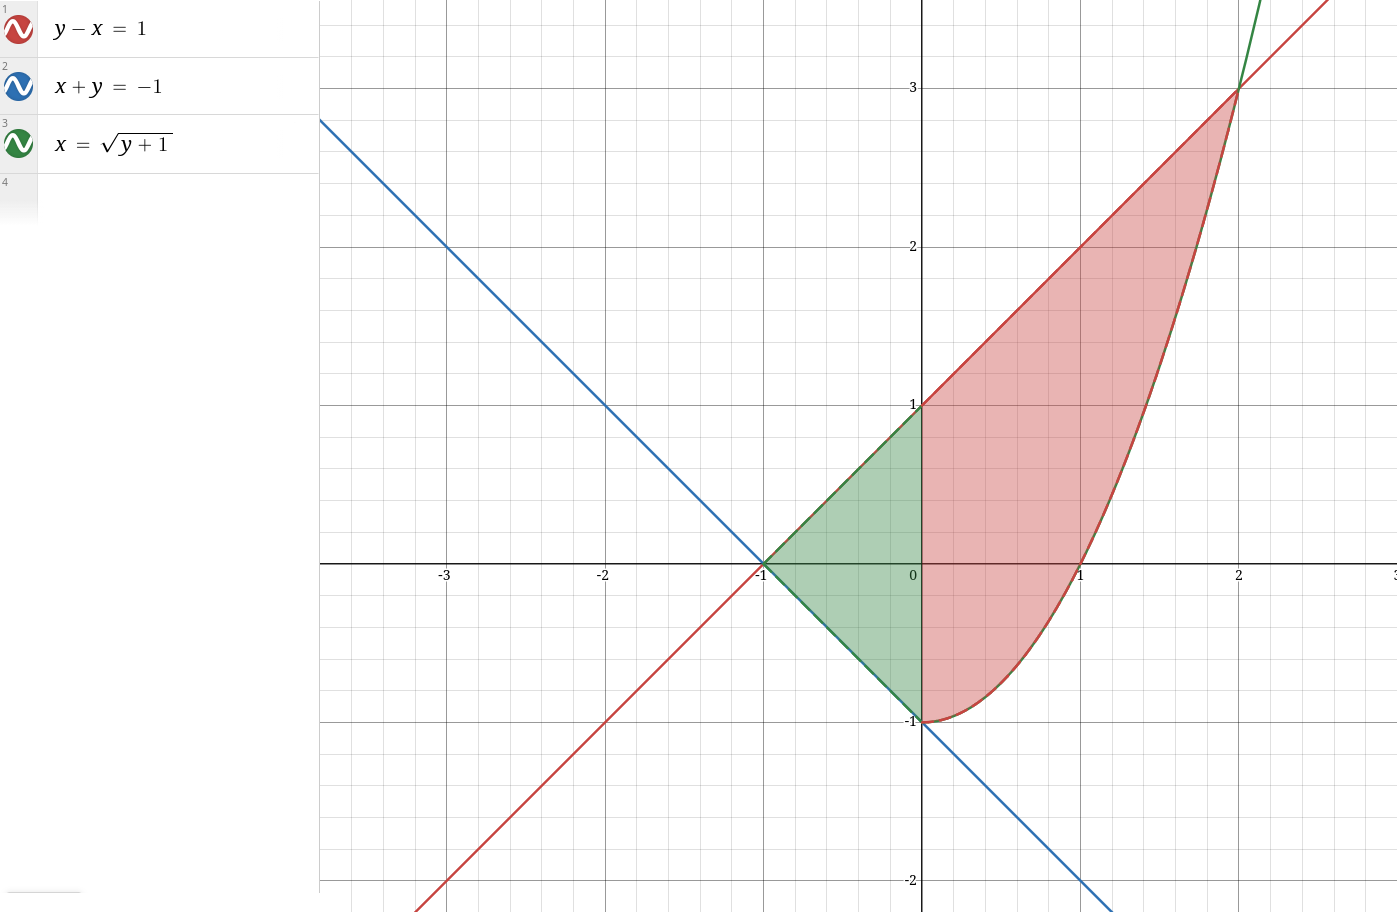
\includegraphics[height=10cm]{graphic.png} \\
    \end{center}
    2) Найдём площадь области $D$: \\
    Для нахождения всей площади области пересечения графиков разделим область на две, найдём их площади и сложим \\
    Первая область (зелёная) $ -1 \leq x \leq 0 $: \\
    \[ S_1 = \int_{-1}^{0} dx \int_{-x-1}^{x+1} dy = \int_{-1}^{0} (x+1 - (-x - 1))dx = \int_{-1}^{0} (2x + 2) dx = (x^2 + 2x) \; \Big|_{-1}^{0} = 1 \]
    Вторая область (красная) $ 0 \leq x \leq 2 $: \\
    \[ S_2 = \int_{0}^{2} dx \int_{x^2-1}^{x+1} dy = \int_{0}^{2} (x+1 - (x^2 - 1))dx = \int_{0}^{2} (-x^2 + x + 2) dx = \Big(\frac{-x^3}{3} + \frac{x^2}{2} + 2x \Big) \; \Big|_{0}^{2} = \frac{-8}{3} + \frac{4}{2} + 4 = \frac{10}{3} \]
    Площадь выделенной области: \\
    $ S = S_1 + S_2 = 1 + \frac{10}{3} = \frac{13}{3} \; \; \; \; \; \; \; $
    Ответ: \boxed{S = \frac{13}{3}} \\
    
\end{flushleft}


\newpage


\begin{flushleft}
    \textbf{Задание 2} \\
    2. Тело T ограничено заданными поверхностями. \\
    1) Сделайте схематический рисунок тела T. \\
    2) С помощью тройного интеграла найдите объем тела T , перейдя к цилиндрическим или сферическим координатам.
    \[ z^2 = 3(x^2 + y^2), \; \; x^2 + y^2 + z^2 = 2z, \; \; x = 0 \; \;
    \text{при} \; x \geq 0, \; 0 \geq z \geq \sqrt{3(x^2 + y^2)} \]

    \textbf{Решение} \\
    1) Схематический рисунок \\
    \begin{center}
        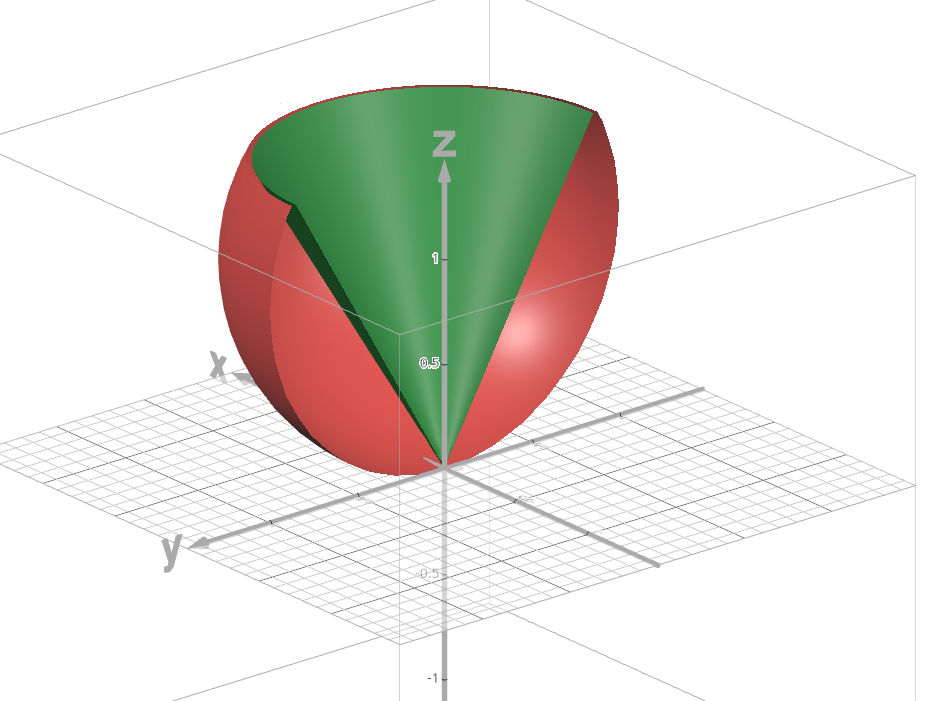
\includegraphics[height=10cm]{graphic1.png} \\
    \end{center}

    2) Найдём объём тела $T$: \\
    Сделаем переход в цилиндрические координаты:
    \[ x = r\cos{\phi} \; \; \; y = r\sin{\phi} \; \; \; z = z\]
    1) Конус: $ z^2 = 3r^2 \rightarrow z = \sqrt{3}r $ \\
    2) Сфера: $ r^2 + z^2 = 2z \rightarrow r = \sqrt{2z - z^2} $ \\
    Пересечение конуса и сферы: $ r^2 = 2z - z^2 = 2\sqrt{3}r - 3r^2 \leftrightarrow r = \frac{\sqrt{3}}{2}; \; \; z = \frac{3}{2} $ \\
    \[ \int_{-\frac{\pi}{2}}^{-\frac{\pi}{2}} \int_{0}^{\frac{3}{2}} \int_{\frac{z}{\sqrt{3}}}^{\sqrt{2z - z^2}} r \; dr \; dz \; d\phi \]
    Итеграл по $r$:
    \[ \int_{\frac{z}{\sqrt{3}}}^{\sqrt{2z - z^2}} r \; dr = \frac{r^2}{2} \Big|_{\frac{z}{\sqrt{3}}}^{\sqrt{2z - z^2}} = \frac{1}{2} \Big( (2z - z^2) - (\frac{z^2}{3}) \Big) = z - \frac{2}{3}z^2 \]
    Интеграл по $z$:
    \[ \int_{0}^{\frac{3}{2}} \Big( z - \frac{2}{3}z^2 \Big) \; dz = \Big( \frac{z^2}{2} - \frac{2}{9}z^3 \Big) \Big|_{0}^{\frac{3}{2}} = \frac{9}{8} - \frac{54}{72} = \frac{3}{8} \]
    Интеграл по $\phi$: 
    \[ \int_{-\frac{\pi}{2}}^{-\frac{\pi}{2}} \frac{3}{8} \; d\phi = \frac{3}{8} \Big( \frac{\pi}{2} - (-\frac{\pi}{2}) \Big) = \frac{3\pi}{8} \]

    Ответ: \boxed{V = \frac{3\pi}{8} } \\

\end{flushleft}



\newpage



\begin{flushleft}

    \textbf{Задание 3}

    С помощью криволинейного интеграла первого рода найдите массу $M$
    дуги плоской материальной кривой, заданной уравнениями: \\
    а) $y = e^x, \qquad \rho(x,y) = 1, \qquad x_1 = \ln\sqrt{3}$, \qquad $x_2 = \ln\sqrt{8}$ \\
    б)
    \[
    \begin{cases}
        x = 2\sqrt{t}, \qquad \rho(x,y) = \sqrt{1 + \frac{3}{4}xy} \\
        y = \frac{2}{3}t\sqrt{t}, \qquad t_1 = 1$, \; $t_2 = 4 \\
    \end{cases} 
    \]

    \textbf{Решение:} \\
    \textbf{Пункт а)} \\
    Для кривой $y = f(x)$ элемент длины дуги:
    \[ dl = \sqrt{1 + (y')^2} \, dx  \]
    \[ y' = (e^x)' = e^x  \Rightarrow \]
    \[ dl = \sqrt{1 + e^{2x}} \, dx \]
    \[ M = \int_{x_1}^{x_2} \rho(x,y) \, dl = \int_{\ln\sqrt{3}}^{\ln\sqrt{8}} \sqrt{1 + e^{2x}} \, dx \]

    Пусть $u = \sqrt{1 + e^{2x}}$. Тогда:
    \[ u^2 = 1 + e^{2x} \quad \Rightarrow \quad e^{2x} = u^2 - 1 \]
    \[ 2u \, du = 2e^{2x} \, dx \quad \Rightarrow \quad dx = \frac{u \, du}{u^2 - 1} \]

    \begin{itemize}
        \item При $x = \ln\sqrt{3}$: $e^{2x} = 3 \Rightarrow u = \sqrt{1 + 3} = 2$
        \item При $x = \ln\sqrt{8}$: $e^{2x} = 8 \Rightarrow u = \sqrt{1 + 8} = 3$
    \end{itemize}
    \[M = \int_2^3 u \cdot \frac{u \, du}{u^2 - 1} = \int_2^3 \frac{u^2}{u^2 - 1} \, du\]
    \[ \frac{u^2}{u^2 - 1} = \frac{u^2 - 1 + 1}{u^2 - 1} = 1 + \frac{1}{u^2 - 1} \]
    \[ \frac{1}{u^2 - 1} = \frac{1}{(u-1)(u+1)} = \frac{1}{2}\left(\frac{1}{u-1} - \frac{1}{u+1}\right)\]
    \[ M = \int_2^3 \left[1 + \frac{1}{2}\left(\frac{1}{u-1} - \frac{1}{u+1}\right)\right] du\]
    \[M = \left[u + \frac{1}{2}\ln\left|\frac{u-1}{u+1}\right|\right]_2^3 \]

    Подставляем верхний предел $u = 3$:
    \[3 + \frac{1}{2}\ln\left(\frac{2}{4}\right) = 3 + \frac{1}{2}\ln\left(\frac{1}{2}\right) = 3 - \frac{1}{2}\ln 2 \]

    Подставляем нижний предел $u = 2$:
    \[
    2 + \frac{1}{2}\ln\left(\frac{1}{3}\right) = 2 - \frac{1}{2}\ln 3
    \]
    \[ M = \left(3 - \frac{1}{2}\ln 2\right) - \left(2 - \frac{1}{2}\ln 3\right) \]
    \[M = 1 + \frac{1}{2}(\ln 3 - \ln 2) = 1 + \frac{1}{2}\ln\left(\frac{3}{2}\right) \]
    Ответ: \boxed{M = 1 + \frac{1}{2}\ln(1.5)} \\

    \vspace{30pt}
    \textbf{Пункт б)}
    \[ \frac{dx}{dt} = \frac{d}{dt}(2\sqrt{t}) = 2 \cdot \frac{1}{2\sqrt{t}} = \frac{1}{\sqrt{t}}\]
    \[ \frac{dy}{dt} = \frac{d}{dt}\left(\frac{2}{3}t^{3/2}\right) = \frac{2}{3} \cdot \frac{3}{2}t^{1/2} = \sqrt{t} \]
    \[dl = \sqrt{\left(\frac{dx}{dt}\right)^2 + \left(\frac{dy}{dt}\right)^2} \, dt = \sqrt{\frac{1}{t} + t} \, dt\]
    \[dl = \sqrt{\frac{1 + t^2}{t}} \, dt = \frac{\sqrt{1 + t^2}}{\sqrt{t}} \, dt\]

    Вычислим произведение $xy$:
        \[xy = 2\sqrt{t} \cdot \frac{2}{3}t\sqrt{t} = \frac{4}{3}t^2\]

    Подставим в формулу плотности:
    \[\rho(x,y) = \sqrt{1 + \frac{3}{4} \cdot \frac{4}{3}t^2} = \sqrt{1 + t^2}\]
    Интеграл:
    \[M = \int_1^4 \rho(x,y) \, dl = \int_1^4 \sqrt{1 + t^2} \cdot \frac{\sqrt{1 + t^2}}{\sqrt{t}} \, dt\]
    \[M = \int_1^4 \frac{(1 + t^2)}{\sqrt{t}} \, dt = \int_1^4 \left(\frac{1}{\sqrt{t}} + \frac{t^2}{\sqrt{t}}\right) dt\]
    \[M = \int_1^4 \left(t^{-1/2} + t^{3/2}\right) dt\]
    \[\int t^{-1/2} \, dt = 2t^{1/2} = 2\sqrt{t}\]
    \[\int t^{3/2} \, dt = \frac{t^{5/2}}{5/2} = \frac{2}{5}t^{5/2} = \frac{2}{5}t^2\sqrt{t}\]

    Подстановка пределов:
    \[M = \left[2\sqrt{t} + \frac{2}{5}t^2\sqrt{t}\right]_1^4\]
    При $t = 4$:\[2\sqrt{4} + \frac{2}{5} \cdot 16 \cdot \sqrt{4} = 2 \cdot 2 + \frac{2}{5} \cdot 16 \cdot 2 = 4 + \frac{64}{5} = 4 + 12.8 = 16.8\]
    При $t = 1$:
    \[2\sqrt{1} + \frac{2}{5} \cdot 1 \cdot \sqrt{1} = 2 + \frac{2}{5} = 2 + 0.4 = 2.4\]
    \[M = 16.8 - 2.4 = 14.4\]
    Ответ: \boxed{$ M = 14.4$} \\
\end{flushleft}


\newpage


\begin{flushleft}
    \textbf{Задание 4} \\
    С помощью криволинейного интеграла первого рода найдите массу $M$ дуги пространственной материальной кривой, заданной уравнениями
    \[
    \begin{cases}
        x = \cos{t}, \\
        y = \sin{t}, \qquad \rho(x, y, z) = \frac{zy}{\sqrt{6 - x^2 - y^2}} \qquad t_1 = 0, \qquad t_2 = \frac{\pi}{2} \\
        z = t, \
    \end{cases}
    \]
    \textbf{Решение:} \\
    \[ M = \int_{t_1}^{t_2} \sqrt{x(t)'^2 + y(t)'^2 + z(t)'^2} \cdot \rho(x, y, z) \; dt \]
    \[ M = \int_{0}^{\frac{\pi}{2}} \sqrt{4\sin^2{t} + \cos^2{t} + 1} \cdot \frac{t \sin{t}}{\sqrt{2 + 3\sin^2{t}}} \; dt = \int_{0}^{\frac{\pi}{2}} \sqrt{2 + 3\sin^2{t}} \cdot \frac{t \sin{t}}{\sqrt{2 + 3\sin^2{t}}} \; dt = \]
    \[ \int_{0}^{\frac{\pi}{2}} = t \sin{t} \; dt\]
    \[
    \begin{cases}
        u = t, \qquad du = dt, \\
        dv = \sin{t}, \qquad v = -\cos{t} \\
    \end{cases}
    \]
    \[ -t\cos{t} - \int_{0}^{\frac{\pi}{2}} -\cos{t} \; dt = (-t\cos{t} + \sin{t})\Big|_0^{\frac{\pi}{2}} = 1 \]
    Ответ: \boxed{M = 1} \\
\end{flushleft}

\end{document}